\documentclass[]{article}
\def\thepage{E\arabic{page}}
\usepackage{color,graphicx}
\usepackage{lastpage}
\usepackage{xspace}
\usepackage{makeidx}
\usepackage{amsmath}
\usepackage[pdflinkmargin=5pt,pdfstartview={FitBH -32768},pdfpagemode=None,plainpages=false]{hyperref}
%\usepackage[screen,article]{pdfscreen}
\hypersetup{pdfauthor=?`\c C\"asar M\"uller n\~ao!`}
\setcounter{tocdepth}{4}
\setcounter{secnumdepth}{4}
\makeindex
\hypersetup{pdftitle=Welcome to the Monkey House}
\newcommand{\ANS}{\textsf{ANSYS}\xspace}
\begin{document}
\tableofcontents
\section*{Abstract}
\addtocontents{toc}{\protect\addvspace{10pt}}
\addcontentsline{toc}{section}{\protect\numberline{}{ABSTRACT}}
\section{A first, simple, section heading}
And some text
\section{A funny \ANS-section with a \texorpdfstring{$\log$}{log}}
Page 1; See \textcolor{red}{page} --\pageref{page2}--
\newpage
Page 2; this is page 2\label{page2}
\newpage
\index{an item on page 3}

\htmladdnormallink{A dummy URL}{http://www.tug.org/A-Fake_URL.html}

\Acrobatmenu{Quit}{End Acrobat Reader}

\Acrobatmenu{FullScreen}{Switch to full screen}

\Acrobatmenu{ZoomIn}{Zoom in}

$\int\!dx$
\section{Yet another ?`\c C\"asar M\"uller n\~ao!`}

\section{Testing Int\'ernal J\oe mps}\label{ss:intjmps}

This is some text and this is a \hypertarget{target}{target}.

\newpage

Now lets jump to \hyperlink{target}{Target}.

Let's try going to Section~\ref{ss:intjmps}

\section{A \ss ection with $\leq$}
xx
xx
\subsubsection{A subsubsection \texorpdfstring{$a+b$}{a+b}}
xx
\paragraph{A paragraph}
xx
\subparagraph{A subparagraph}
xxx
Pictures:

Normal 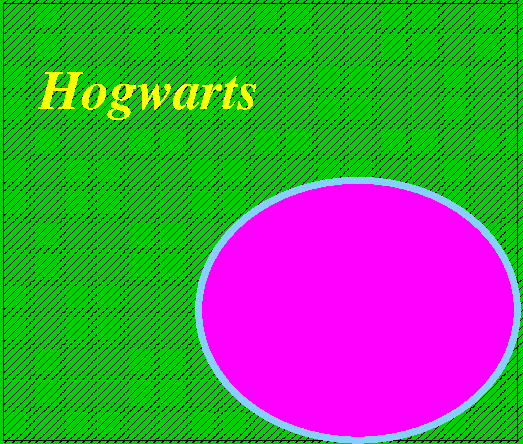
\includegraphics{hog}

Scaled 0.75 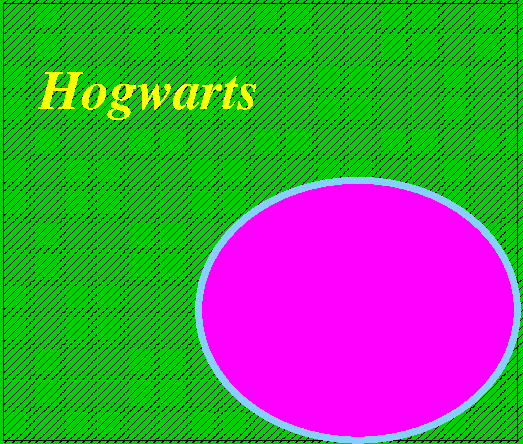
\includegraphics[scale=0.75]{hog}

Width 1in height 0.5in
  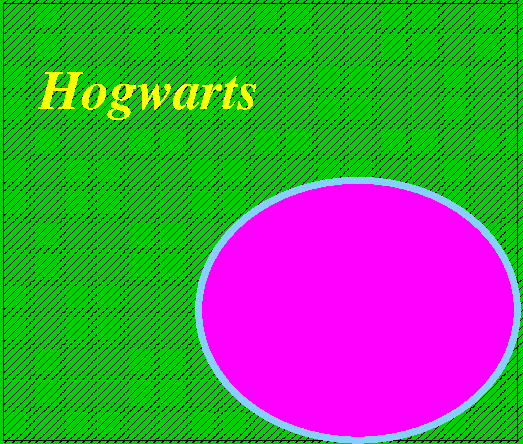
\includegraphics[width=1in,height=0.5in]{hog}

Rotated 50 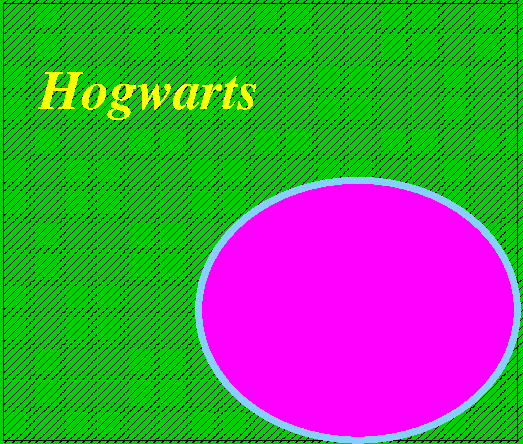
\includegraphics[scale=0.5,angle=50]{hog}

Rotated -50 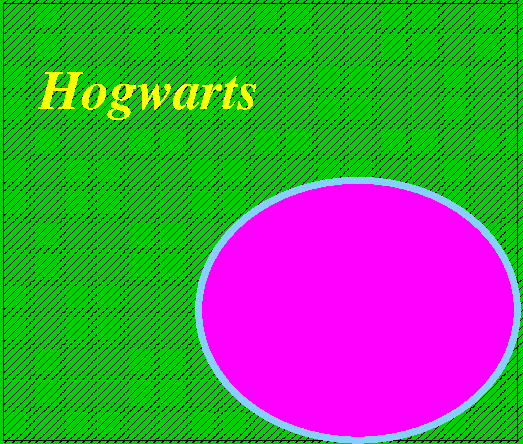
\includegraphics[scale=0.5,angle=-50]{hog}


\section{Testing External Jumps}\label{ss:extjmps}

\begin{enumerate}

\item Jump to an external: The jump
\href{file:test7#TestTarget}{target} should open test7.pdf on
page 2, 
\item  Jump to an external: The jump
\href{file:test7#page.1}{page 1} should open test7.pdf on
page 1.

%\item Jump to an relative external strange file
%\href{/D/srahtz/skills.doc}{destination}

\href{run:picture.eps}{a PS file to launch}

\href{run:fontman.exe}{an application}

\href{run:e:\string\\mdraw\string\\mdraw.exe#picture.eps}{a PS file to launch (2)}
\end{enumerate}
\printindex
\clearpage
\end{document}



